

\subsection{Grafiken und Animationen}

%\begin{figure}[H]
 %  \centering
 %   \label{fig:mine_exterior_concept}
  %  \caption{Concept Art -> Finale Grafik}
   % \subfloat[][]{\fbox{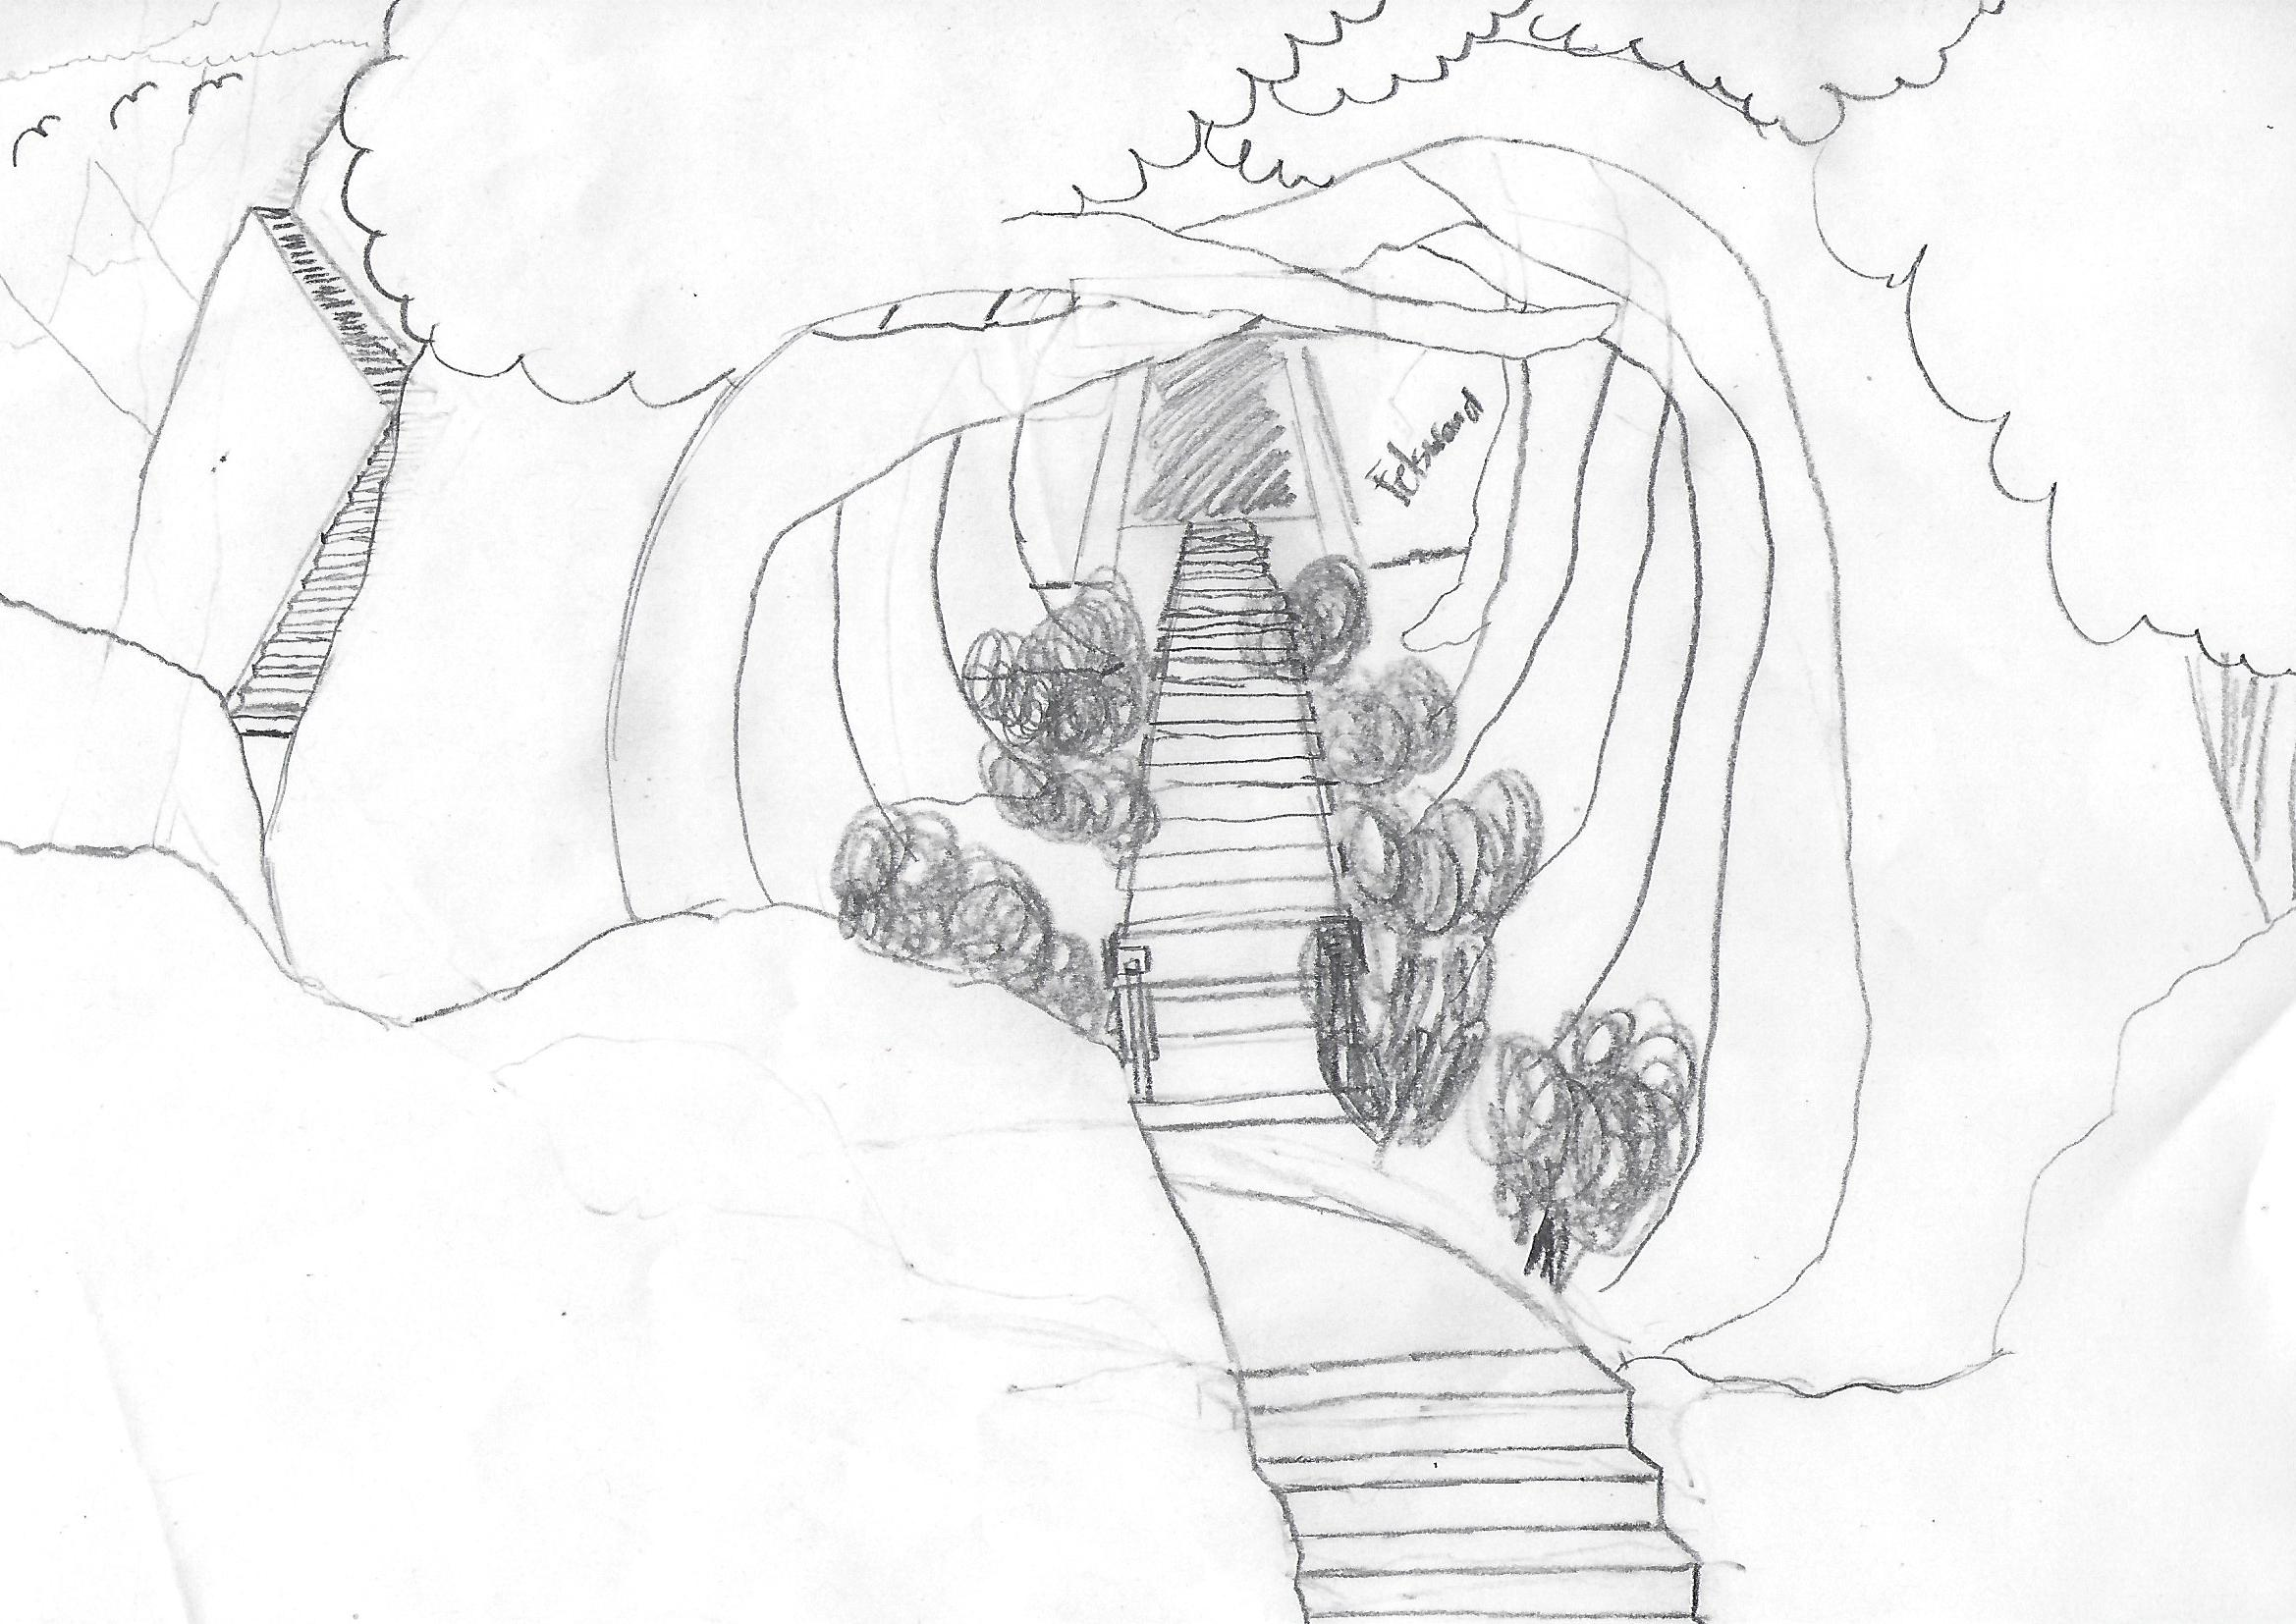
\includegraphics[width=0.5\linewidth]{mine_exterior_concept}}}
  %  \subfloat[][]{\fbox{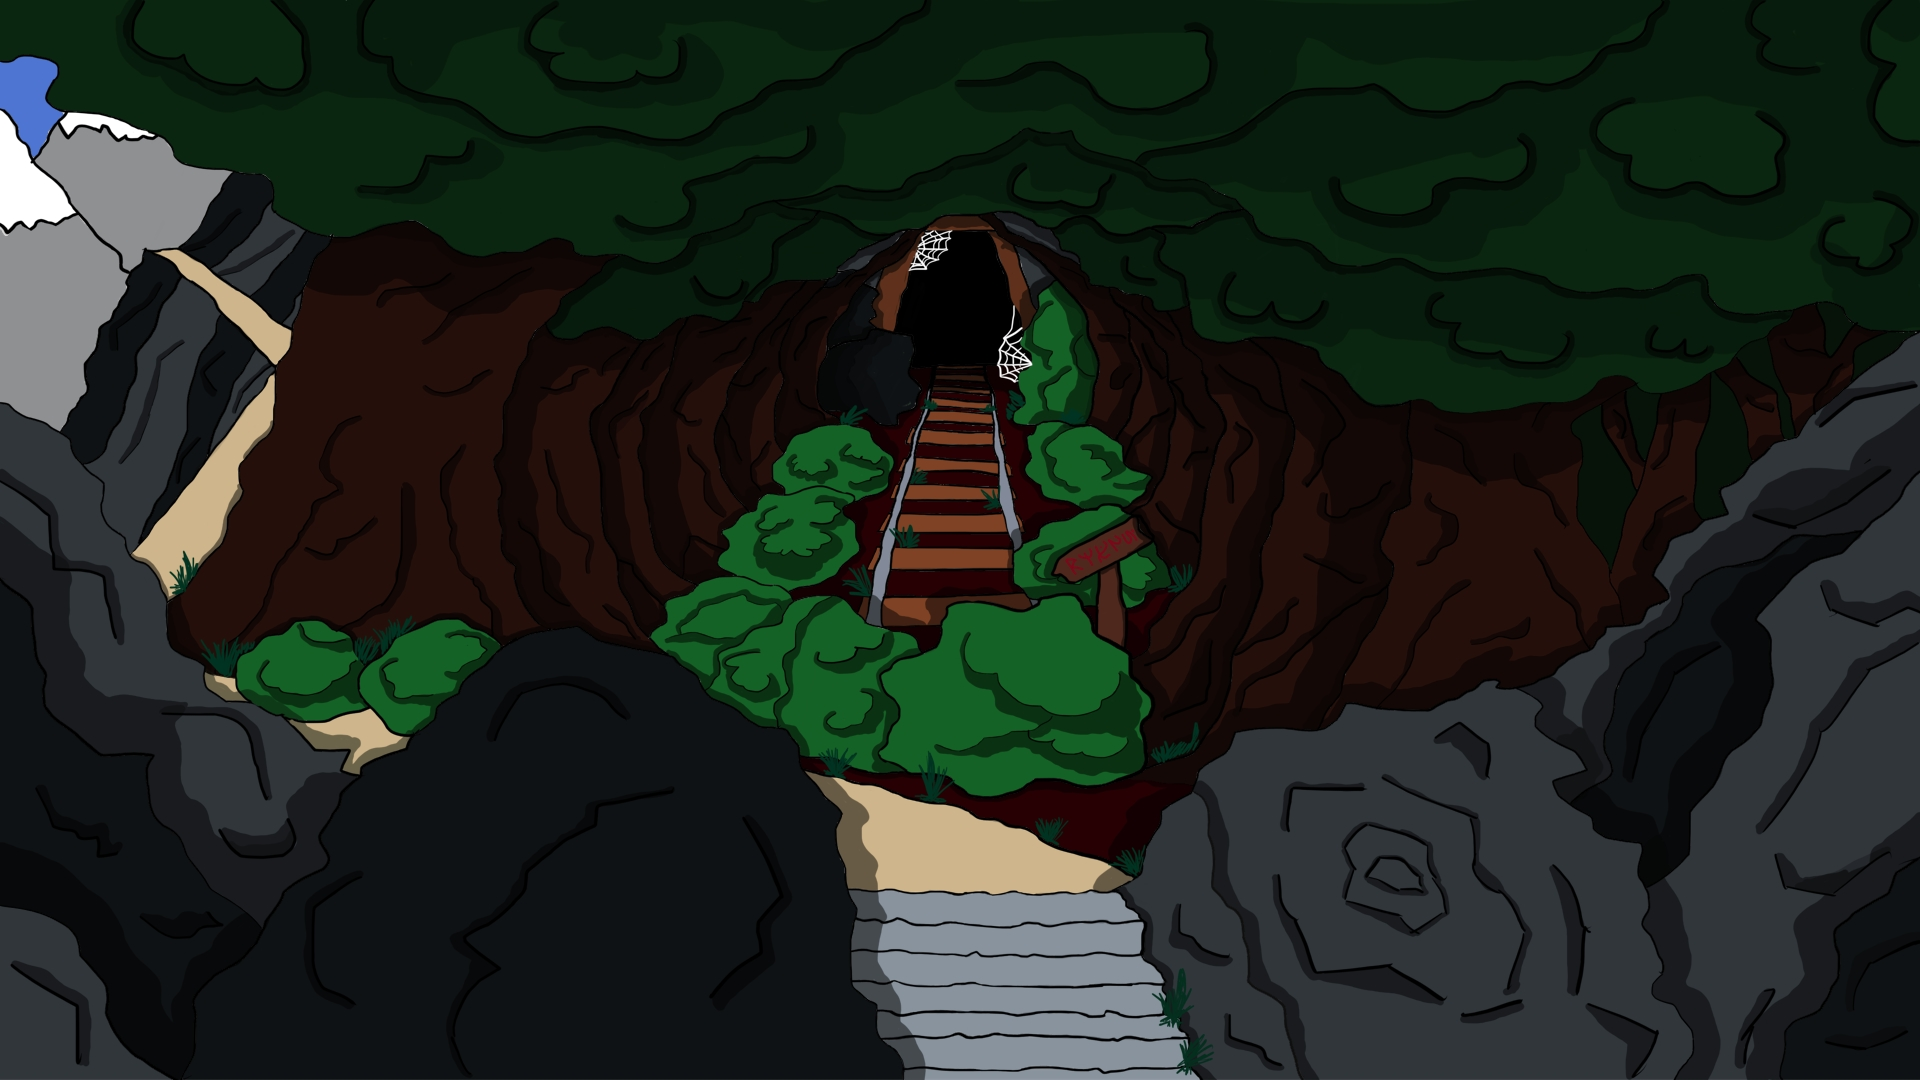
\includegraphics[width=0.5\linewidth]{mine_exterior_final}}}
%\end{figure}

Jede der Spielszenen hat drei Grafik-Assets: eine Intrografik für die Szenenlobby, einen Hintergrund für den Kampfbildschirm und eine Bossgegner-Grafik mit 2D-Animationen. Zudem kommt noch eine weitere Grafik für die Weltkarte hinzu. Diese Letztere, Intro und Hintergrund besitzen das JPG-Bildformat. Die Bossgegner-Grafik dagegen ist ein MP4-Video.
\\Für das JPG-Format entschieden wir uns hauptsächlich auf Grund der im Vergleich zu PNG geringeren Dateigröße. Da es sich bei allen Grafiken, um rein statische Bilder handelt, erschien der Komprimierungsverlust von jpg vernachlässigbar. Zudem wurde für die Bilder keine Hintergrund-Transparenz benötigt.
Alle Grafiken wurden in einer Auflösung von 3840x2160 (Ultra-HD) gezeichnet und dann entweder so verwendet oder auf 1920x1080 (Full-HD) herabskaliert. 

Für die Erstellung der Grafik-Assets und Animationen wurden das freie Zeichen- und 2D-Animationsprogramm \textit{Krita}\footnote{siehe https://krita.org/en/} und ein Grafiktablet verwendet (in der folgenden Abbildung beispielhaft das Standard-UI von Krita).   

\begin{figure}[H]
    \centering
    \caption{Krita Standard-UI}
    \label{fig:krita_ui_example}
    \fbox{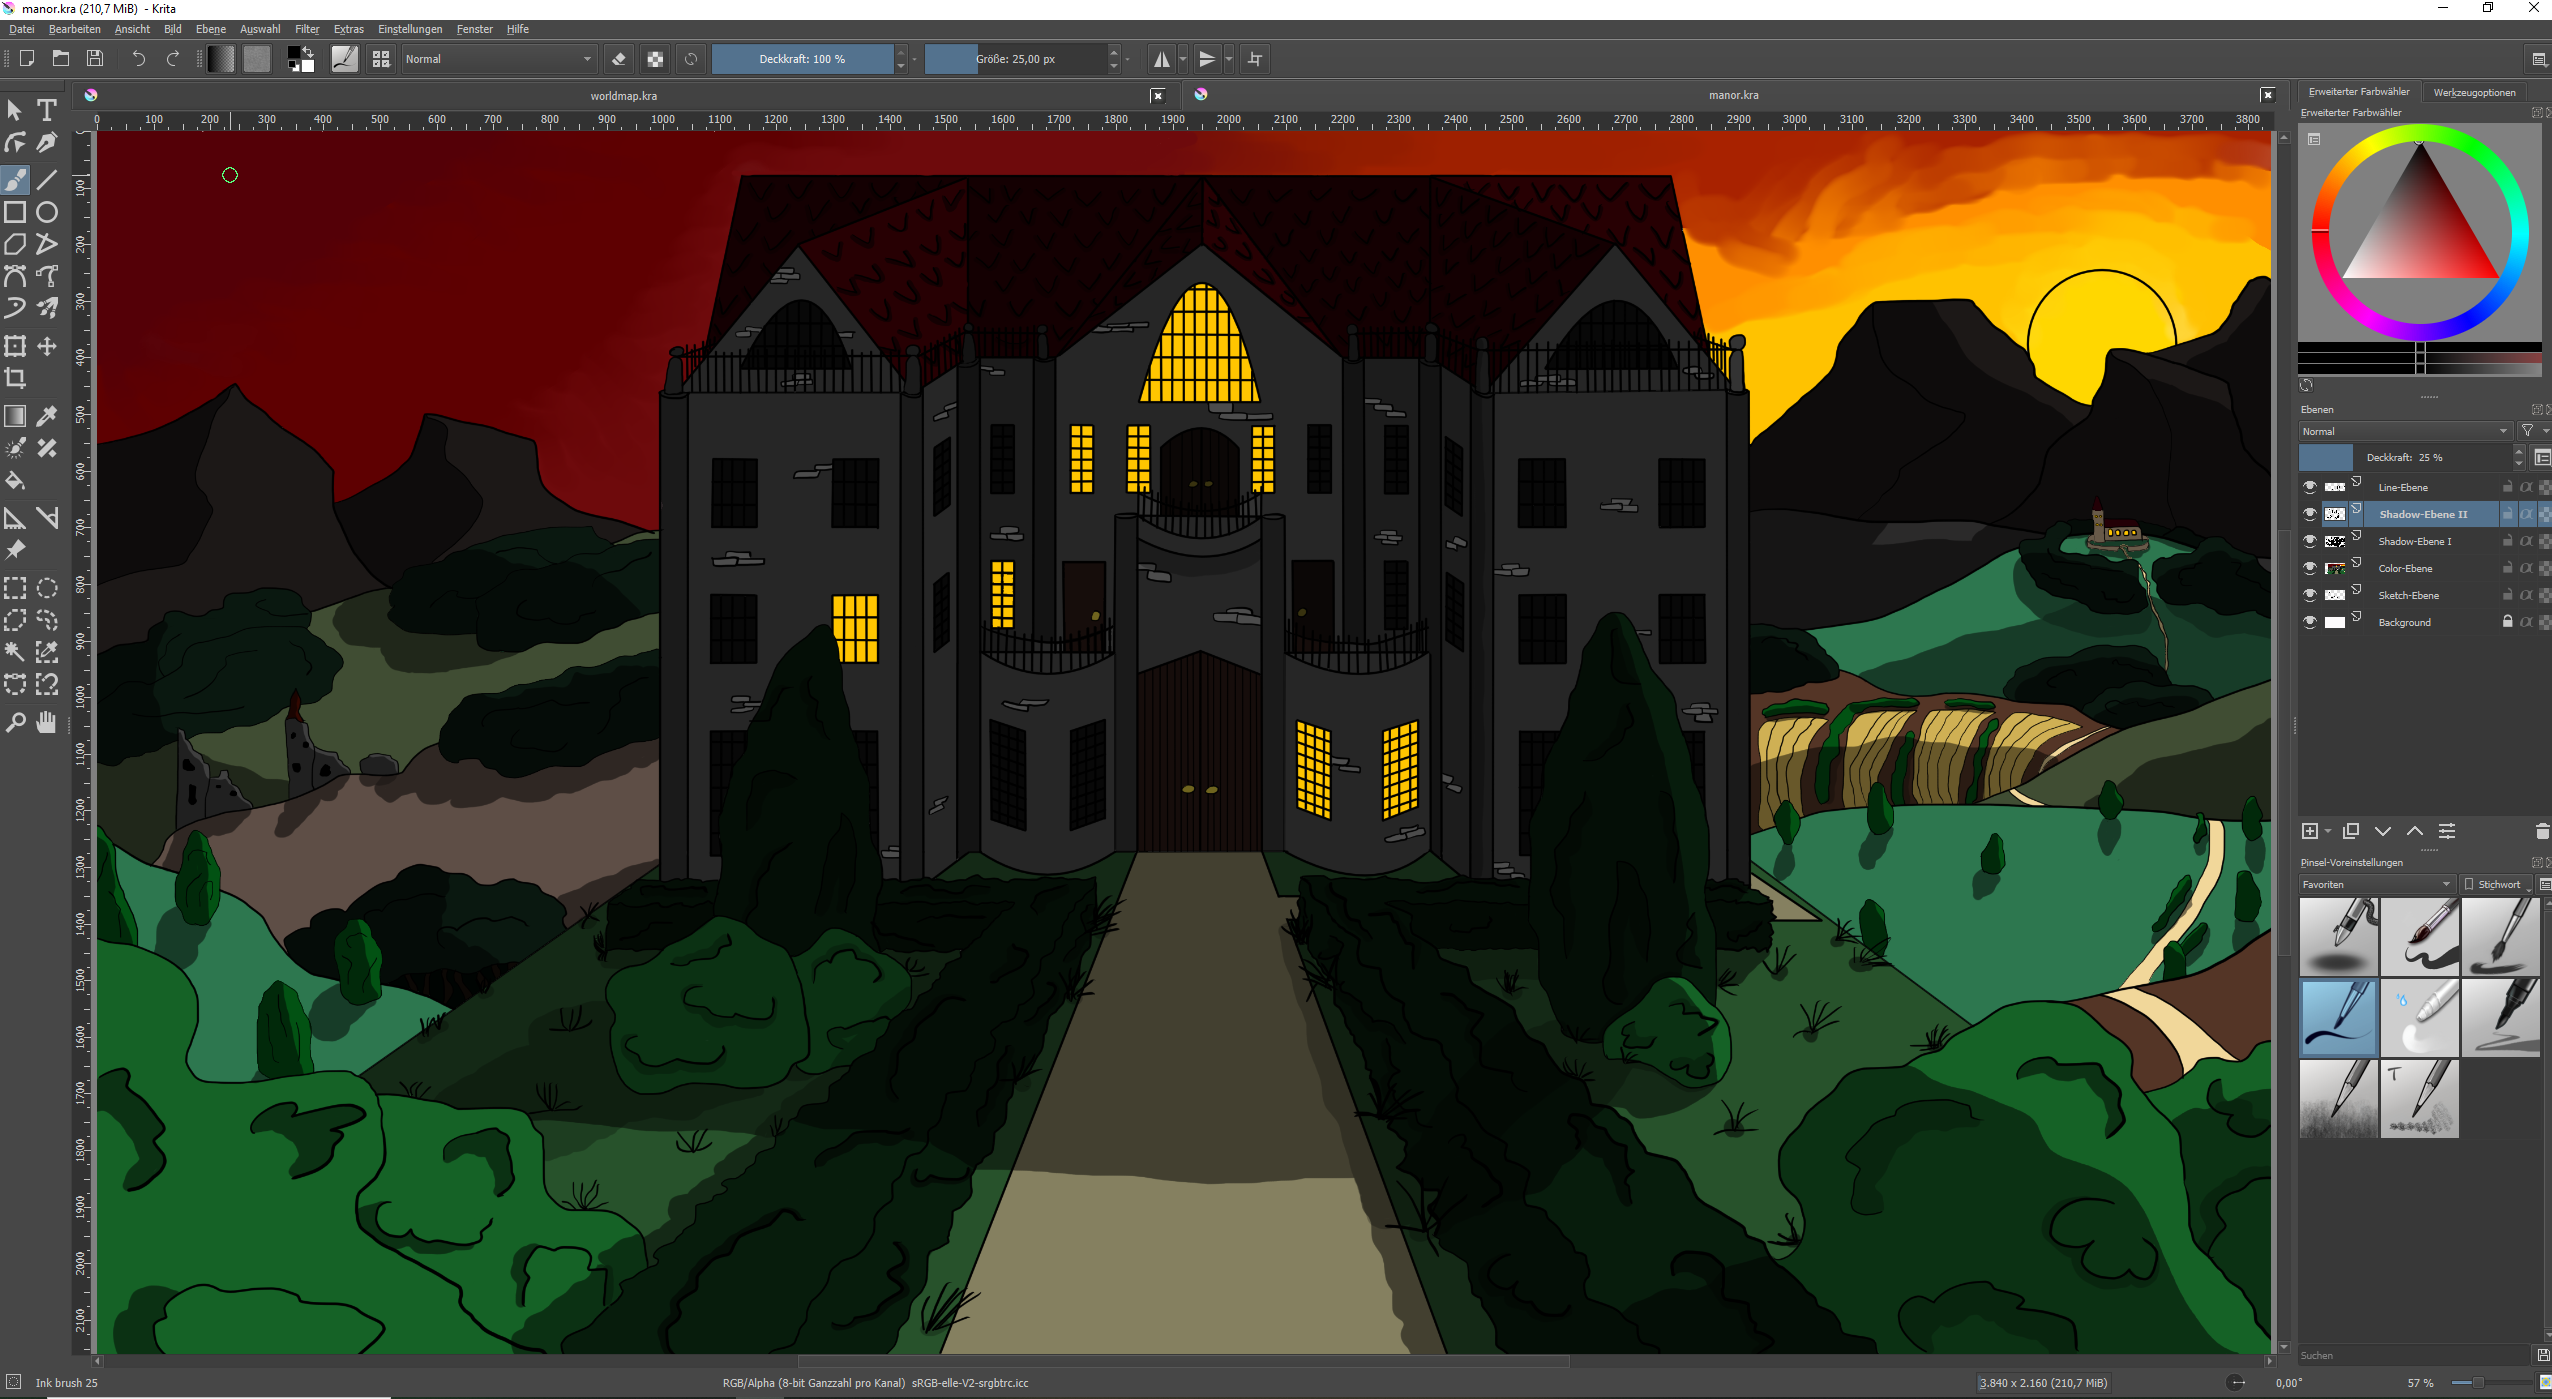
\includegraphics[width=1\textwidth]{krita_ui_example}}
\end{figure}

Die Grafiken wurden hierbei mithilfe der softwareeigenen Ebenenhierarchie systematisch wie folgt aufgebaut: 

Eine Konzeptzeichnung bildet die unterste Ebene mit einer vergleichsweise geringen Deckkraft (\enquote{Sketch-Ebene}). Darüber folgt die \enquote{Linien-Ebene}, auf der auf Basis der Skizze eine vollständige Strichzeichnung mit maximaler Deckkraft angefertigt wird. Diese bildet die oberste Ebene und alle folgenden Ebenen werden aufsteigend zwischen diesen beiden positioniert. Durch eine sorgfältige Linienführung auf dieser Ebene kann das Fülltool auf der nun folgenden \enquote{Farb-Ebene} effektiv genutzt werden. Den Abschluss bilden ein oder zwei \enquote{Schatten-Ebenen}, die mit einer Deckkraft von 50\% bzw. 25\% über der eigentlichen Kolorierung liegen. 

Im Falle der Bossgegner-Grafiken wird dieses Konzept noch um drei Gruppen ergänzt, welche jeweils alle Ebenen in sich zusammenfassen. Es gibt eine Gruppe für das Hintergrundbild, eine Gruppe für die nicht-aninimierten Teile des Bossgegners und eine Gruppe für die eigentlichen Animationen.
Zum Vergleich ist im Folgenden eine Abbildung dieses Aufbaus zu sehen (hier beispielhaft eine Grafik mit 2D-Animation):

\begin{figure}[H]
    \centering
    \caption{Ebenenkonzept für die Grafiken}
    \label{fig:krita_layer_example}
    \fbox{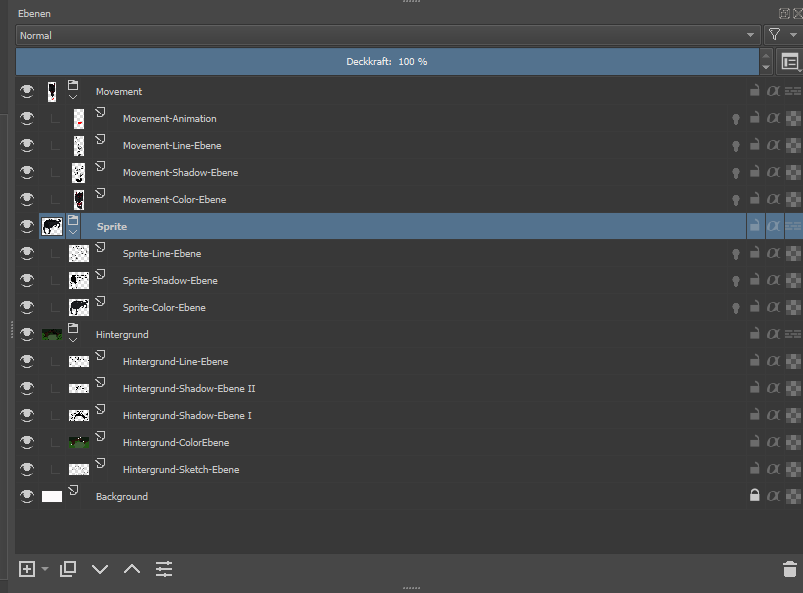
\includegraphics[width=0.7\textwidth]{krita_layer_example}}
\end{figure}

\pagebreak
Dieses Konzept brachte eine erhebliche Flexibilität mit sich. Es war uns damit möglich effizient Änderungen an separaten Teilen der Grafiken durchzuführen, mit der Farbgebung zu experimentieren und nachträglich neue Details einzubringen. Zudem konnten Hintergrundbilder und Bossgrafiken als eine Datei erstellt werden und dann durch Ausblenden verschiedenener Ebenen individuell exportiert werden. Auch der Animationsprozess wurde durch diese Technik deutlich erleichtert. 

Für die Realisierung der 2D-Animationen bietet \textit{Krita} ein dediziertes User-Interface (siehe Abbildung unten). Die Ebenen können hier je nach Bedarf zusammen oder einzeln animiert werden. Dazu werden sie unabhängig voneinander in die Animationsframes kopiert und gegebenenfalls verändert. Im unten zu sehenden Beispiel werden die Ebenengruppen \enquote{Sprite} (nicht-animierter Teil der Bossgegner-Grafik) und \enquote{Movement} (eigentliche Animation) über 10 Frames hinweg durch sukzessive Erhöhung der Deckkraft eingeblendet, um den Effekt eines plötzliches Erscheinens aus Unsichtbarkeit zu erzielen. Danach wird in der \enquote{Movement}-Gruppe über 29 Frames eine Flügelbewegung realisiert. Die Animation wurde dann mit einer Bildwiederholrate von 10 Frames per Second gerendert und als MP4-Video in Ultra-HD und Full-HD exportiert. 

\begin{figure}[H]
    \centering
    \caption{Krita Animation UI}
    \label{fig:krita_animation_example}
    \fbox{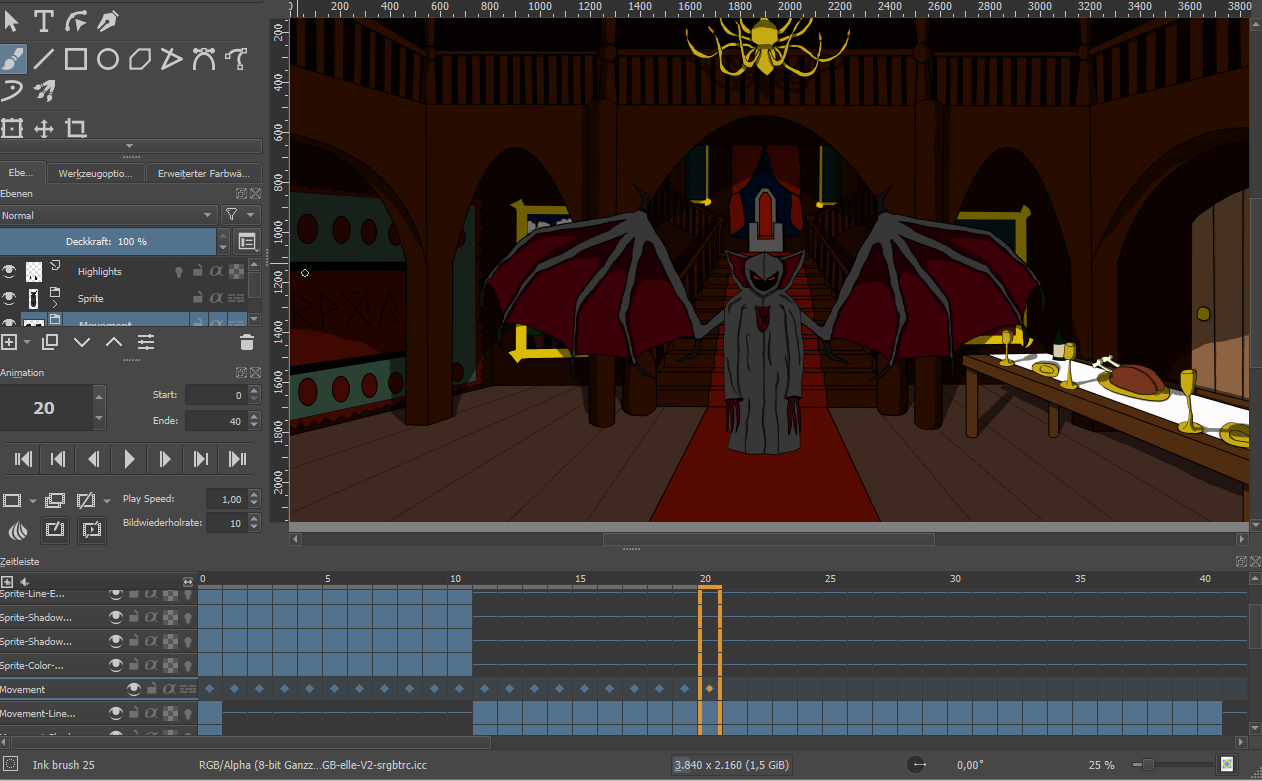
\includegraphics[width=1\textwidth]{krita_animation_example}}
\end{figure}

Die Separierung der Grafiken in animierte und nicht-animierte Teile, stellte bei der eigentlichen Animation eine erhebliche Arbeitserleichterung dar. Viele Veränderungen konnten durch verschieben vorher definierter Abschnitte erreicht werden und mussten nicht pro Frame neu gezeichnet werden (teilweise wurde dies aber trotzdem nötig). Aufgrund des trotz diesen Vorteils immer noch erheblichen Arbeitsaufwandes für vergleichsweise wenige Frames, entschieden wir aber es bei eher rudimentären Animationen zu belassen. Eine Realisierung in 30 Frames per Second beispielsweise wäre and dieser Stelle unverhältnismäßig aufwendig gewesen.

\subsection{Frontend-Design}
    - Design
        - Stil (8-Bit Ära RPG/Adventure)
        - CSS Framework
        - Aufbau des Frontends (HTML-Seiten)
        - Design der einzelnen Seiten 

    - Technisches
        - Worldmap Areas -> SVG-Grafiken

    